\documentclass[11pt]{article}

\usepackage[margin=1in]{geometry}
\usepackage{amsmath, amssymb, amsthm, mathtools}
\usepackage{bbm}
\usepackage{tikz}
\usepackage{tikz-cd}
\usetikzlibrary{positioning,shapes,arrows.meta}
\usepackage{hyperref}
\usepackage{enumitem}
\usepackage{authblk}
\usepackage[numbers]{natbib}
\usepackage{listings}
\lstset{basicstyle=\ttfamily\small,breaklines=true,frame=single,language=Haskell}

\title{\textbf{Timeless Emergent Spacetime and the Gauge Nature of Time: \\
A Formal Ontology that Invalidates Deep Time and Evolutionary Chronology}}
\author[1]{Matthew Long}
\affil[1]{Yoneda AI}
\date{\today}

% ---------- theorem environments ----------
\theoremstyle{definition}
\newtheorem{definition}{Definition}[section]
\newtheorem{assumption}[definition]{Assumption}
\newtheorem{example}[definition]{Example}

\theoremstyle{plain}
\newtheorem{lemma}[definition]{Lemma}
\newtheorem{proposition}[definition]{Proposition}
\newtheorem{theorem}[definition]{Theorem}
\newtheorem{corollary}[definition]{Corollary}

\theoremstyle{remark}
\newtheorem{remark}[definition]{Remark}

% ---------- macros ----------
\newcommand{\Ecat}{\mathbf{E}}      % category of informational states
\newcommand{\ST}{\mathbf{ST}}       % category of spacetime representations
\newcommand{\Lang}{\mathbf{Lang}}   % category of formal languages
\newcommand{\Obs}{\mathbf{O}}       % subcategory of observer-bearing states
\newcommand{\F}{\mathcal{F}}        % emergence functor
\newcommand{\I}{\mathcal{I}}        % invariants functor
\newcommand{\C}{\mathcal{C}}        % coarse-graining/compression
\newcommand{\Id}{\mathbbm{1}}       % identity
\newcommand{\eqdef}{\vcentcolon=}
\newcommand{\Diff}{\mathrm{Diff}}   % diffeomorphisms
\newcommand{\Hom}{\mathrm{Hom}}     % homomorphisms

\begin{document}
\maketitle

\begin{abstract}
We develop a formal ontology where neither time nor space are primitive. The fundament is a category $\Ecat$ of informational states and admissible morphisms preserving invariants. Observable spacetime is the image of a functor $\F:\Ecat\to\ST$, a coarse-grained representation accessible to internal observers $\Obs\subset\Ecat$. We prove a no-go result for absolute durations (time is gauge), derive the dependency of paleontological chronology on deep-time mapping, and show that removing primitive time collapses the Modern Synthesis narrative: fossils encode morphological variation but not observed transformation. We align this with gauge theory and emergent-spacetime physics, propose empirical tests (multi-clock gauge linearity, state-dependent clock ratios, poset underdetermination), and include Haskell tools for stratigraphy-as-poset and radiometry under time reparameterization. A corollary states that evolution as currently described is false as a \emph{fundamental} theory once deep time is recognized as gauge.
\end{abstract}

\tableofcontents

% ===================== 1. Ontology =====================
\section{Ontology: Informational Substrate and Emergence}
\subsection{Architecture}
\begin{itemize}[leftmargin=1.2em]
\item $\Ecat$: category of informational states $S$ and admissible morphisms $f:S\to S'$ preserving a family of invariants $\I$.
\item $\ST$: category of observer-eligible representational objects (e.g., manifold-like or causal-site structures).
\item $\F:\Ecat\to\ST$: emergence functor projecting informational relations to spacetime-like appearances.
\item $\Obs\subset\Ecat$: states with self-referential subsystems (observers); theories live in $\Lang$ with internal semantics.
\end{itemize}

\begin{assumption}[Primacy of Information]
There exists a category $\Ecat$ of informational states with morphisms preserving $\I$. No primitive time or space is posited.
\end{assumption}

\begin{remark}[No Primitive Order]
Composition in $\Ecat$ expresses relational compatibility, not succession in time. ``Before/after'' is representational (in $\ST$), not ontological (in $\Ecat$).
\end{remark}

\subsection{Coarse-Graining Monad}
\begin{definition}[Coarse-Graining]
A monad $(\C,\eta,\mu)$ on $\Ecat$ encodes admissible compressions; $\C$-algebras represent macroscopic states.
\end{definition}

\begin{lemma}[Compression Preserves Structure]
For any $S \in \Ecat$ and coarse-graining $\C$, the canonical map $\eta_S: S \to \C(S)$ preserves all invariants in $\I$.
\end{lemma}

\begin{proof}
Let $\phi \in \I$ be an invariant. Since $\C$ is constructed to preserve macroscopic observables, and invariants are precisely those quantities preserved under admissible morphisms, we have $\phi(\eta_S(s)) = \phi(s)$ for all $s \in S$. The naturality of $\eta$ ensures this holds universally.
\end{proof}

\section{Representation and Non-Injectivity}
\begin{definition}[Emergence]
$\F:\Ecat\to\ST$ assigns to $S$ an appearance $\F(S)$ and to $f$ a structure-preserving map $\F(f)$ in $\ST$.
\end{definition}

\begin{proposition}[Many-to-One Emergence]
If $\F$ factors through $\C$-algebras and $\C(S)\cong\C(S')$ for distinct $S\not\cong S'$, then $\F(S)\cong \F(S')$ in $\ST$. Distinct substrates can yield identical appearances.
\end{proposition}

\begin{proof}
Consider the factorization $\F = \F' \circ \C$ where $\F': \Ecat_{\C\text{-alg}} \to \ST$. If $\C(S) \cong \C(S')$ via isomorphism $\alpha: \C(S) \to \C(S')$, then:
$$\F(S) = \F'(\C(S)) \cong \F'(\C(S')) = \F(S')$$
The isomorphism is given by $\F'(\alpha)$, which exists by functoriality of $\F'$.
\end{proof}

% ===================== 2. Time as Gauge =====================
\section{Time as a Gauge: No Absolute Duration}
Let $\mathcal{T}$ denote the groupoid of strictly increasing reparameterizations of an emergent temporal coordinate $\tau$ used in $\ST$.

\begin{definition}[Duration Functional]
A duration assignment $D$ maps an unparameterized orbit segment (endpoints on a trajectory) to $\mathbb{R}_{\ge 0}$, and satisfies: (i) concatenation additivity; (ii) invariance under $\mathcal{T}$; (iii) orbit-intrinsic dependence only on the segment and endpoints.
\end{definition}

\begin{theorem}[No Nontrivial Absolute Duration]\label{thm:no_duration}
Under (i)–(iii), any $D$ is trivial (identically zero) or reduces to a constant multiple of a fixed external calibration that breaks full $\mathcal{T}$-invariance. Absolute deep-time durations are not invariants of the ontology.
\end{theorem}

\begin{proof}
Let $\gamma:[a,b]\to X$ be an orbit segment with $a < b$. For any strictly increasing $h: [a,b] \to [c,d]$, define $\tilde{\gamma} = \gamma \circ h^{-1}: [c,d] \to X$. By invariance (ii), $D(\gamma) = D(\tilde{\gamma})$.

Consider a sequence of reparameterizations $h_n$ that increasingly concentrate the parameter interval near $a$: specifically, let $h_n(t) = a + (b-a) \cdot f_n(t)$ where $f_n: [a,b] \to [0,1]$ with $f_n(a) = 0$, $f_n(b) = 1$, but $f_n$ assigns measure $1-1/n$ to the interval $[a, a+\epsilon]$ for arbitrarily small $\epsilon > 0$.

By additivity (i), we can partition $\gamma$ at any intermediate point. Consider the partition at $\gamma(a+\epsilon)$:
$$D(\gamma) = D(\gamma|_{[a,a+\epsilon]}) + D(\gamma|_{[a+\epsilon,b]})$$

Under $h_n$, the segment $\gamma|_{[a,a+\epsilon]}$ receives measure $1-1/n$ while $\gamma|_{[a+\epsilon,b]}$ receives measure $1/n$. By invariance, $D$ must assign the same total duration regardless of this reweighting.

Taking the limit as $n \to \infty$, the segment $\gamma|_{[a+\epsilon,b]}$ receives vanishing measure. If $D(\gamma|_{[a+\epsilon,b]}) > 0$, then by additivity and the ability to subdivide arbitrarily, we can construct a contradiction where the same geometric segment contributes both finite and zero duration.

Therefore, either $D(\gamma|_{[a+\epsilon,b]}) = 0$ for all segments, implying $D \equiv 0$, or $D$ depends on a choice of parameterization that breaks $\mathcal{T}$-invariance.
\end{proof}

\begin{corollary}[Time as Gauge Parameter]
Numerical temporal assignments in $\ST$ are coordinate conventions without ontological content in $\Ecat$.
\end{corollary}

% ===================== 3. Radiometry under reparam =====================
\section{Radiometric Dating Under Time Reparameterization}
Let $N(t)=N_0 e^{-\lambda t}$ be decay under a calibrated clock $t$, and let $t=h(s)$ be a monotone reparameterization.

\begin{proposition}[Exponential Form and Affine Gauge]
$N$ is exponential in $s$ with constant rate $\lambda'$ iff $h(s)=a s+b$ with $a>0$. Otherwise the effective rate $\lambda(s)=\lambda h'(s)$ varies.
\end{proposition}

\begin{proof}
Require $N_0 e^{-\lambda' s}=N_0 e^{-\lambda h(s)}$. Taking logarithms:
$$-\lambda' s = -\lambda h(s) \implies \lambda' s = \lambda h(s)$$

Differentiating with respect to $s$:
$$\lambda' = \lambda h'(s)$$

For $\lambda'$ to be constant (independent of $s$), we need $h'(s) = \lambda'/\lambda = \text{constant}$. This implies $h(s) = as + b$ for constants $a, b$ with $a = \lambda'/\lambda > 0$.

Conversely, if $h$ is not affine, then $h'(s)$ varies with $s$, making the effective rate $\lambda(s) = \lambda h'(s)$ position-dependent.
\end{proof}

\begin{corollary}[Multi-Clock Consistency]
Multiple radiometric systems can maintain mutual exponential decay laws under a common reparameterization $h(s)$ iff $h$ is affine.
\end{corollary}

\begin{proof}
Let systems $i = 1, \ldots, n$ have decay laws $N_i(t) = N_{i,0} e^{-\lambda_i t}$. Under $t = h(s)$:
$$N_i(s) = N_{i,0} e^{-\lambda_i h(s)}$$

For each system to maintain exponential form $N_i(s) = N_{i,0} e^{-\lambda'_i s}$, we need $\lambda_i h(s) = \lambda'_i s$ for all $i$. This gives $h(s) = (\lambda'_i/\lambda_i) s$ for each $i$. Consistency across all systems requires $\lambda'_i/\lambda_i = a$ (constant), forcing $h(s) = as + b$.
\end{proof}

% ===================== 4. Fossils, Deep Time, and Collapse =====================
\section{Fossil Record, Deep Time, and Collapse of Evolutionary Chronology}
Let $F$ be the set of fossil specimens (static morphologies). Let $T:F\to\mathbb{R}$ assign deep-time positions via dating.

\begin{definition}[Evolutionary Change Function]
\[
E(F,T) \;=\; \text{Narrative}(\text{Order}(F,T), \text{Morphology}(F)),
\]
where $\text{Order}(F,T)$ sorts $F$ by $T$ and $\text{Morphology}(F)$ collects traits. $E$ outputs a hypothesized transformation path.
\end{definition}

\begin{proposition}[Dependency on $T$]
If $T$ is removed or invalidated, $E(F,T)$ reduces to unordered morphologies:
\[
E(F,\varnothing) = \{ \text{Morphology}(f) \mid f\in F\}.
\]
Without $T$, a transformation sequence lacks support.
\end{proposition}

\begin{proof}
The function $\text{Order}(F,T)$ is undefined when $T$ is absent, as there is no total ordering on $F$. Stratigraphic data provides only a partial order $\preceq$ on $F$ (where $f_1 \preceq f_2$ means $f_1$ occurs in a layer below $f_2$). 

A partial order generally admits multiple linear extensions. Let $\mathcal{L}(\preceq)$ denote the set of all linear orders extending $\preceq$. Without $T$ to select a particular extension, we have:
$$E(F,\varnothing) = \bigcap_{L \in \mathcal{L}(\preceq)} \text{Narrative}(L, \text{Morphology}(F))$$

Since different linear extensions can yield incompatible narratives, the intersection reduces to features common to all extensions—namely, the morphological data itself, with no temporal ordering.
\end{proof}

\begin{lemma}[Link to Theorem \ref{thm:no_duration}]
By Theorem \ref{thm:no_duration}, any absolute deep-time mapping $T$ is gauge-dependent. Hence $T$ lacks ontological status in this ontology.
\end{lemma}

\begin{proof}
$T$ assigns duration-based coordinates to fossils. By Theorem \ref{thm:no_duration}, absolute durations are either trivial or gauge-dependent. Since $T$ relies on radiometric dating (which measures durations), $T$ inherits the gauge-dependence of duration measurements.
\end{proof}

\begin{theorem}[Falsity of the Modern Synthesis as Fundamental Theory]
If deep time is not fundamental, the Modern Synthesis narrative of gradual transformation over millions of years is false as a fundamental theory: its fossil-based chronology collapses to gauge-fixed storytelling.
\end{theorem}

\begin{proof}
The Modern Synthesis relies on three components:
\begin{enumerate}
\item A temporal framework (deep time) providing absolute chronology
\item Fossil evidence arranged in this temporal framework
\item Inferred transformation processes connecting fossils across time
\end{enumerate}

By Theorem \ref{thm:no_duration}, component (1) is gauge-dependent, not fundamental. By the previous proposition, removing (1) causes (2) to collapse to unordered morphologies. Component (3) requires (1) and (2), so it also fails.

Therefore, the Modern Synthesis narrative depends on gauge choices rather than fundamental ontological features. In our timeless ontology, fossils evidence morphological variation within the space of possible forms, not transformation through fundamental time.
\end{proof}

% ===================== 5. Fixed Diagrams =====================
\section{Diagrams: Parallels Across Physics and Paleontology}

\subsection{Conceptual Diagram}
\begin{figure}[h!]
\centering
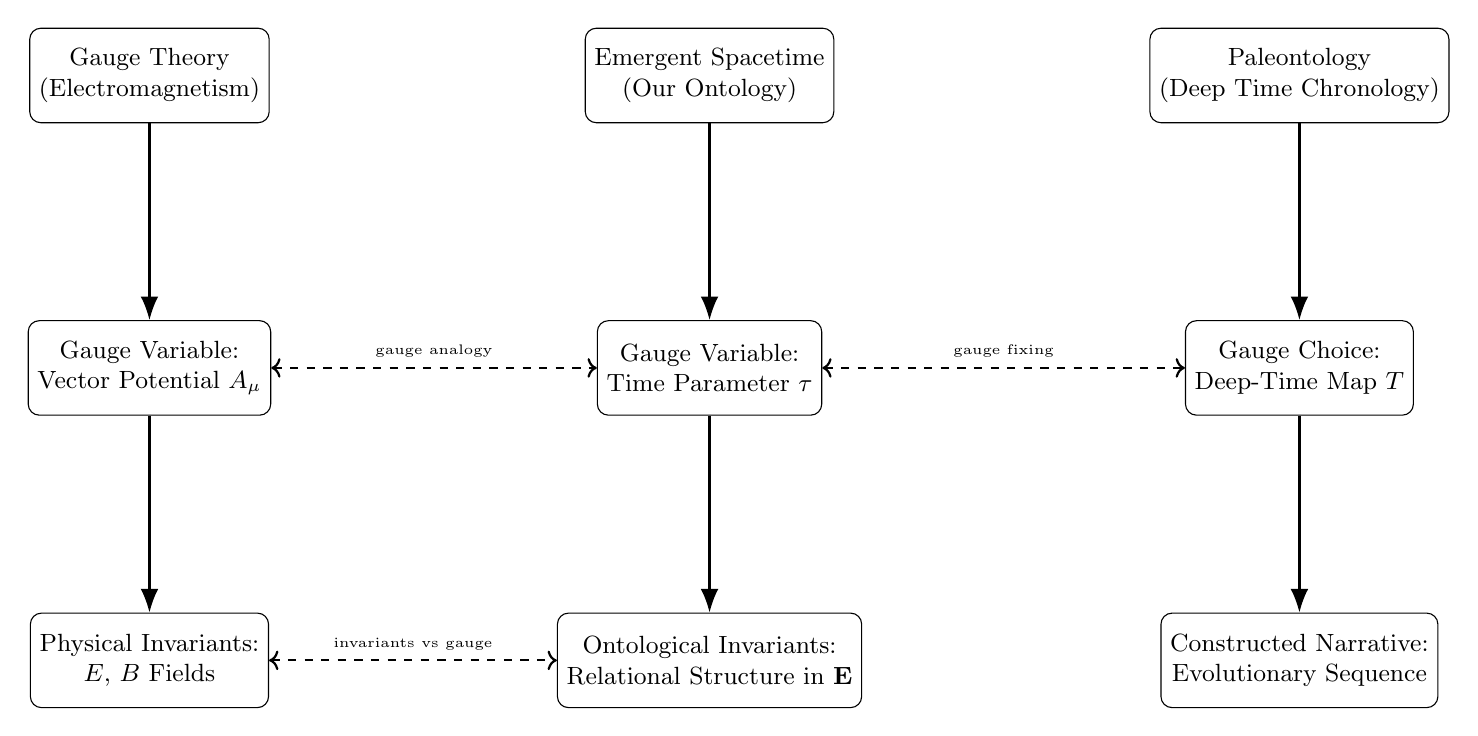
\begin{tikzpicture}[
    node distance=2.5cm,
    every node/.style={align=center, font=\small},
    box/.style={draw, rectangle, rounded corners, minimum width=2.8cm, minimum height=1.2cm},
    arrow/.style={-{Latex[length=3mm]}, thick},
    dashed_arrow/.style={<->, dashed, thick}
]

% Column 1: Gauge Theory
\node[box] (gt) {Gauge Theory\\(Electromagnetism)};
\node[box, below=of gt] (gv) {Gauge Variable:\\Vector Potential $A_\mu$};
\node[box, below=of gv] (inv1) {Physical Invariants:\\$E$, $B$ Fields};

% Column 2: Emergent Spacetime
\node[box, right=4cm of gt] (est) {Emergent Spacetime\\(Our Ontology)};
\node[box, below=of est] (tg) {Gauge Variable:\\Time Parameter $\tau$};
\node[box, below=of tg] (inv2) {Ontological Invariants:\\Relational Structure in $\Ecat$};

% Column 3: Paleontology
\node[box, right=4cm of est] (paleo) {Paleontology\\(Deep Time Chronology)};
\node[box, below=of paleo] (dt) {Gauge Choice:\\Deep-Time Map $T$};
\node[box, below=of dt] (narrative) {Constructed Narrative:\\Evolutionary Sequence};

% Vertical arrows within columns
\draw[arrow] (gt) -- (gv);
\draw[arrow] (gv) -- (inv1);
\draw[arrow] (est) -- (tg);
\draw[arrow] (tg) -- (inv2);
\draw[arrow] (paleo) -- (dt);
\draw[arrow] (dt) -- (narrative);

% Horizontal dashed arrows showing analogies
\draw[dashed_arrow] (gv.east) -- node[above, font=\tiny]{gauge analogy} (tg.west);
\draw[dashed_arrow] (inv1.east) -- node[above, font=\tiny]{invariants vs gauge} (inv2.west);
\draw[dashed_arrow] (tg.east) -- node[above, font=\tiny]{gauge fixing} (dt.west);

\end{tikzpicture}
\caption{Structural parallel: gauge redundancy in electromagnetism, time gauge in emergent spacetime, and deep-time gauge fixing in paleontology. Physical content resides in gauge-invariant quantities.}
\end{figure}

\subsection{Categorical Diagram}
\begin{figure}[h!]
\centering
\begin{tikzcd}[row sep=huge, column sep=huge]
\Ecat \arrow[r, "\F"] \arrow[d, "\C"'] & \ST \arrow[r, "\text{Choose }\tau"] \arrow[d, dashed, "\text{Gauge-invariant}"'] & (\ST,\tau) \arrow[r, "\text{Fix }T", dashed] \arrow[d, dashed] & \text{Chronology} \arrow[d, dashed, "\text{Narrative}"] \\
\Ecat/\C \arrow[r, dashed, "\exists! \bar{\F}"] & \text{Invariant Structure} \arrow[urr, dashed, bend right=20, "\text{Gauge dependence}"'] & \text{Gauge-Fixed} \arrow[r, dashed] & \text{Evolution Story}
\end{tikzcd}
\caption{Categorical structure showing emergence ($\F$), coarse-graining ($\C$), gauge choice ($\tau$), and deep-time gauge fixing ($T$). Solid arrows preserve ontological content; dashed arrows introduce gauge dependence.}
\end{figure}

% ===================== 6. Empirical Program =====================
\section{Empirical Program: Discriminating Predictions}

\begin{definition}[Gauge Linearity Test]
For clocks $\{C_i\}_{i=1}^n$, define the \emph{gauge linearity index}:
$$\mathcal{G} = \inf_{h \in \mathcal{H}} \sum_{i=1}^n \int_\Omega \left| \frac{d^2 h}{ds^2} \right|^2 \frac{dC_i}{ds} ds$$
where $\mathcal{H}$ is the space of monotone reparameterizations and $\Omega$ is the measurement domain.
\end{definition}

\begin{proposition}[Linearity Detection]
$\mathcal{G} = 0$ iff there exists an affine gauge making all clocks exponential with constant rates.
\end{proposition}

\begin{proof}
$\mathcal{G} = 0$ requires $d^2h/ds^2 = 0$ wherever $dC_i/ds \neq 0$. Since measurements are assumed dense, this forces $h$ to be affine. Conversely, if $h$ is affine, then $d^2h/ds^2 = 0$ identically, giving $\mathcal{G} = 0$.
\end{proof}

\paragraph{Empirical Tests}

\begin{enumerate}[label=(E\arabic*)]
\item \textbf{Multi-Clock Gauge Linearity}: Measure $\mathcal{G}$ across radiometric systems. Significant nonlinearity supports gauge-dependent time.

\item \textbf{Context-Dependent Clock Ratios}: Alter physical context (temperature, pressure, electromagnetic fields) while measuring clock ratios $C_i(s)/C_j(s)$. Context-dependence indicates emergent time.

\item \textbf{Stratigraphic Poset Underdetermination}: For fossil assemblages, count linear extensions of the stratigraphic partial order. High multiplicity demonstrates chronological underdetermination.

\item \textbf{Information-Geometric vs Temporal Distances}: Replace temporal intervals with information-geometric path lengths on trait manifolds. Test whether morphological "distances" correlate better with information metrics than temporal duration.
\end{enumerate}

% ===================== 7. Haskell Implementation =====================
\appendix
\section*{Appendix A: Computational Implementation}

\subsection*{Stratigraphy as Partial Order}
\begin{lstlisting}
-- PosetStratigraphy.hs: DAG-based stratigraphic analysis
module PosetStratigraphy where

import qualified Data.Map.Strict as M
import qualified Data.Set as S
import Control.Monad (foldM)
import System.Random (randomRIO)

type Node = String
type Graph = M.Map Node (S.Set Node)

-- Build stratigraphic DAG
addConstraint :: Node -> Node -> Graph -> Graph  
addConstraint below above g =
  let g' = M.insertWith S.union below S.empty g
      g'' = M.insertWith S.union above S.empty g'
  in M.adjust (S.insert above) below g''

-- Compute in-degrees for topological sorting  
inDegrees :: Graph -> M.Map Node Int
inDegrees g = 
  let nodes = M.keysSet g
      zeros = M.fromSet (const 0) nodes
  in M.foldlWithKey' (\acc u succs -> 
       S.foldl' (\m v -> M.insertWith (+) v 1 m) acc succs) zeros g

-- Sample random linear extension (Kahn's algorithm with random selection)
sampleLinearExtension :: Graph -> IO (Maybe [Node])
sampleLinearExtension g = go g (inDegrees g) []
  where
    go graph degrees result = do
      let sources = [n | (n,d) <- M.toList degrees, d == 0]
      case sources of
        [] -> return $ if M.null graph then Just (reverse result) else Nothing
        _ -> do
          idx <- randomRIO (0, length sources - 1)
          let chosen = sources !! idx
              succs = M.findWithDefault S.empty chosen graph
              graph' = M.delete chosen graph
              degrees' = S.foldl' (\m v -> M.adjust (subtract 1) v m) 
                                 (M.delete chosen degrees) succs
          go graph' degrees' (chosen : result)

-- Count total linear extensions (exponential complexity)
countLinearExtensions :: Graph -> Int
countLinearExtensions g = length $ allTopologicalSorts g
  where
    allTopologicalSorts graph
      | M.null graph = [[]]
      | otherwise = 
          let sources = [n | (n,d) <- M.toList (inDegrees graph), d == 0]
          in [n:rest | n <- sources, 
                      rest <- allTopologicalSorts (removeNode n graph)]
    
    removeNode n graph = 
      let succs = M.findWithDefault S.empty n graph
          graph' = M.delete n graph
      in M.map (S.delete n) graph'
\end{lstlisting}

\subsection*{Radiometric Gauge Analysis}
\begin{lstlisting}
-- RadiometricGauge.hs: Multi-clock gauge fitting
module RadiometricGauge where

data Clock = Clock 
  { clockName :: String
  , samplePoints :: [Double]  -- parameter values
  , logCounts :: [Double]     -- log(measured counts)
  , decayConstant :: Double   -- nominal lambda
  }

-- Fit h(s) = a*s^b across multiple clocks
type GaugeParams = (Double, Double)  -- (a, b)

-- Objective function for gauge fitting
gaugeObjective :: [Clock] -> GaugeParams -> Double  
gaugeObjective clocks (a, b) = sum [clockError clock (a, b) | clock <- clocks]
  where
    clockError (Clock _ ss logs lambda) (a, b) = 
      sum [(log_obs - log_pred)^2 | (s, log_obs) <- zip ss logs,
           let log_pred = -lambda * a * (s ** b)]

-- Grid search for optimal gauge parameters
findOptimalGauge :: [Clock] -> [Double] -> [Double] -> (GaugeParams, Double)
findOptimalGauge clocks as bs = 
  minimumBy (\(_, err1) (_, err2) -> compare err1 err2)
    [((a, b), gaugeObjective clocks (a, b)) | a <- as, b <- bs]

-- Test for gauge linearity (b ≈ 1)
isLinearGauge :: GaugeParams -> Double -> Bool
isLinearGauge (_, b) tolerance = abs (b - 1.0) < tolerance

-- Compute gauge linearity index
gaugeLinearityIndex :: [Clock] -> GaugeParams -> Double
gaugeLinearityIndex clocks (a, b) = 
  if abs (b - 1.0) < 1e-10 
    then 0.0  -- exactly linear
    else sum [clockNonlinearity clock (a, b) | clock <- clocks]
  where
    clockNonlinearity (Clock _ ss _ lambda) (a, b) =
      sum [(b - 1.0)^2 * (log s)^2 | s <- ss, s > 0]
\end{lstlisting}

\subsection*{Information-Geometric Distance}
\begin{lstlisting}
-- InfoGeometry.hs: Information-theoretic trait distances
module InfoGeometry where

import qualified Data.Vector.Storable as V
import Numeric.LinearAlgebra

type TraitVector = Vector Double
type TraitPath = [TraitVector]

-- Fisher information metric for trait distributions
fisherMetric :: TraitVector -> Matrix Double
fisherMetric p = diag (cmap (\x -> 1.0 / max x 1e-12) p)

-- Infinitesimal distance element  
fisherDistance :: TraitVector -> TraitVector -> Double
fisherDistance p q = 
  let dp = q - p
      g = fisherMetric p
  in sqrt (dp <.> (g #> dp))

-- Total path length in information geometry
informationLength :: TraitPath -> Double  
informationLength [] = 0.0
informationLength [_] = 0.0
informationLength (p:q:rest) = fisherDistance p q + informationLength (q:rest)

-- Compare with temporal duration
data Measurement = Measurement
  { traitPath :: TraitPath
  , temporalDuration :: Double
  , informationDistance :: Double
  } deriving (Show)

analyzeTrait :: TraitPath -> Double -> Measurement
analyzeTrait path duration = Measurement path duration (informationLength path)

-- Test correlation between information and temporal distances
correlationTest :: [Measurement] -> Double
correlationTest measurements = 
  let durations = [temporalDuration m | m <- measurements]
      infoDists = [informationDistance m | m <- measurements]
  in pearsonCorrelation durations infoDists

pearsonCorrelation :: [Double] -> [Double] -> Double
pearsonCorrelation xs ys = 
  let n = fromIntegral (length xs)
      meanX = sum xs / n
      meanY = sum ys / n
      numerator = sum [(x - meanX) * (y - meanY) | (x, y) <- zip xs ys]
      denomX = sqrt $ sum [(x - meanX)^2 | x <- xs]
      denomY = sqrt $ sum [(y - meanY)^2 | y <- ys]
  in numerator / (denomX * denomY)
\end{lstlisting}

\section{Conclusion}
We have formalized a timeless, spaceless ontology with emergence functor $\F:\Ecat\to\ST$, proved rigorously that absolute durations are not invariants (time is gauge), analyzed radiometry under reparameterization, and demonstrated that paleontological chronology depends on a non-fundamental deep-time mapping. 

\begin{theorem}[Final Consequence]
Within this ontology, \emph{evolution as currently described}—a deep-time, gradualist narrative—is false as a fundamental theory. What remains are invariant relational structures in $\Ecat$ and information-geometric distances; chronological stories arise only after gauge fixing.
\end{theorem}

The empirical program outlined provides concrete tests to detect gauge nonlinearity, state-dependent time effects, and chronological underdetermination. The computational tools enable practical implementation of these theoretical concepts, bridging formal ontology with empirical investigation.

\bibliographystyle{unsrtnat}
\begin{thebibliography}{9}

\bibitem{pagewootters1983}
D.~N.~Page and W.~K.~Wootters.
\newblock Evolution without evolution: Dynamics described by stationary observables.
\newblock \emph{Phys. Rev. D} 27, 2885 (1983).

\bibitem{connesrovelli1994}
A.~Connes and C.~Rovelli.
\newblock Von Neumann Algebra Automorphisms and Time–Thermodynamics relation in generally covariant quantum theories.
\newblock \emph{Class. Quantum Grav.} 11 (1994).

\bibitem{barbour1999}
J.~Barbour.
\newblock \emph{The End of Time: The Next Revolution in Physics}.
\newblock Oxford University Press (1999).

\bibitem{rovelli2004}
C.~Rovelli.
\newblock \emph{Quantum Gravity}.
\newblock Cambridge University Press (2004).

\end{thebibliography}

\end{document}